\documentclass[12pt,  openany]{book}
\pagestyle{plain}
\usepackage[utf8]{inputenc}
\usepackage[T1]{fontenc}

\usepackage{extsizes}
\usepackage[english,russian]{babel}
\usepackage{geometry}
\usepackage{graphicx}
\usepackage{float}
\usepackage{hyphsubst}
\usepackage{svg}
\usepackage{tempora}
\usepackage{amsmath}
\usepackage{relsize}
\usepackage{listings}
\usepackage[nottoc,notlot,notlof,numbib]{tocbibind}
\usepackage{natbib}
\usepackage{indentfirst}
\usepackage{titlesec}
\titleformat{\chapter}[display]
  {\normalfont\bfseries}{}{0pt}{\Huge}
\usepackage{listings}
\usepackage{xcolor}
\usepackage{hyperref}
\hypersetup{
    colorlinks,
    citecolor=black,
    filecolor=black,
    linkcolor=black,
    urlcolor=black
}

\definecolor{codegreen}{rgb}{0,0.6,0}
\definecolor{codegray}{rgb}{0.5,0.5,0.5}
\definecolor{codepurple}{rgb}{0.58,0,0.82}
\definecolor{backcolour}{rgb}{0.98,0.98,0.98}

\lstdefinestyle{mystyle}{
    frame=single,
    aboveskip=5mm,
    belowskip=5mm,
    backgroundcolor=\color{backcolour},   
    commentstyle=\color{codegreen},
    keywordstyle=\color{blue},
    numberstyle=\small\color{codegray},
    stringstyle=\color{codepurple},
    basicstyle=\ttfamily\footnotesize,
    breakatwhitespace=false,         
    breaklines=true,                 
    captionpos=b,                    
    keepspaces=true,                 
    numbers=left,                    
    numbersep=7pt,                  
    showspaces=false,                
    showstringspaces=false,
    showtabs=false,                  
    tabsize=2
}

\lstset{style=mystyle}
  
\geometry{
    a4paper,
    left=30mm,
    top=20mm,
    right=15mm,
    bottom=20mm
}
\linespread{1.5}
\setlength{\parindent}{1.25cm}

\begin{document}
\chapter{Аннотация}
В современном мире очень много информации. И если Вы разрабатываете любое приложение, рано или поздно перед Вами встает вопрос - как и где хранить информацию ваших пользователей и вашего приложения. Здесь Вам на помощью приходит огромное количество уже существующих баз данных. И зачастую данных бывает настолько много, что неоправданно хранить их на одном компьютере. Тогда Вы используете распределенную базу данных. К современным распределенным базам данных предъявляется ряд требований. Одно из таких требований - согласованность данных в каждый момент времени. 
\par Конечно же, разработчиков распределенных систем интересует вопрос: как быстро и легко тестировать согласованность системы? И как же удостовериться в том, что реализация транзакции (наш основной инструмент работы  с данными) удовлетворяет своим основным свойствам? 
\par Один из инструментов для проверки гарантий согласованности, который практически не имеет аналогов, это инструмент хаос-тестирования Jepsen. 
\par В этой работе мы  узнали больше о моделях согласованности распределенных систем. 
Изучили различные феномены, нарушающие гарантии согласованности и изолированности. А также мы познакомились с  Jepsen и принципами его работы. 
\par Кроме того, мы попробовали самостоятельно проанализировать Azure Cosmos DB с помощью Jepsen. В 15\% историй мы обнаружили G2-item аномалию, которая,хоть и не противоречит заявленной в документации изоляции моментальных снимков, нарушает также заявленное в документации <<full ACID>> свойство транзакций.


\setcounter{page}{2}
\tableofcontents
\clearpage



\chapter{Введение}

Существует спрос на инструменты проверки согласованности транзакций, так  как базы данных не обеспечивают тот уровень согласованности, на который претендуют.  Почему? Чем они могут быть полезны?
\begin{itemize}
\item Пользователю(разработчику приложения, хранящего свои данные в базе данных) хочется научиться понимать про ту или иную базу данных, насколько она соответствует документации (это необходимо для того, чтобы выбрать базу данных, которая больше всего подходить для потребностей пользователя-разработчика);
\item Удобный инструмент для тестирования согласованности может существенно помочь на этапе разработки распределенных систем, возможно, стать одним из этапов CI/CD процесса;
\item Jepsen проводит свои исследования независимо и в соответствии с их этической политикой. Это вносит большой вклад в сообщество, помогает в развитии и совершенствовании распределенных систем.
\end{itemize}
Большинство распределенных систем стремятся к достижению баланса между временем выполнения операций и согласованностью.  Один из инструментов для проверки гарантии согласованности - это инструмент хаос-тестирования Jepsen.  Хаос-тестирование ---  это тестирование путем внесения в систему незапланированных сбоев \cite{chaosTesting}.  Наблюдая за поведением системы, можно понять, как сделать распределенную систему более надежной. Хаос тестирование это важная часть тестирования, потому что помогает выявить состояния гонки (race condition), которые сложно иначе обнаружить в процессе разработки.

\section{Цели работы}
\begin{itemize}
  \item Получить опыт работы с выбранным инструментом проверки свойств транзакций (Jepsen);
  \item Изучить выполненные данным инструментом исследования различных баз данных;
  \item Исследовать с помощью выбранного инструмента реальную базу данных (Azure Cosmos DB), которая еще не была проанализирована;
  \item Сравнить уровень согласованности, заявленный в документации, и уровень, установленный с помощью тестов.
\end{itemize}

\section{Основные понятия}
Введем основные понятия,  необходимые в дальнейшем.

\emph{Параллельная система} ---  это система, состоящая из независимых компонент, которые могут выполнять некоторые операции одновременно.

\emph{Распределенная система} ---  это тип параллельных систем, который представляет собой систему с несколькими независимыми компонентами, которые расположены на разных узлах в компьютерной сети.  Эти узлы способны обмениваться данными, а также они кооридинируют свои действия так, чтобы для конечного пользователя распределенная система работала как единая согласованная система.  Система имеет логическое стостояние, которое меняется с течением времени. 

\emph{Хаос-тестирование \cite{chaosTesting}} ---  это тестирование путем внесения в распределенную систему незапланированных сбоев.

\emph{Процесс} ---  это логически однопоточная программа, которая способна выполнять некоторые операции. 

\emph{Операция} --- переход из одного состояние в другое. 

\emph{Атомарная операция} --- операция в общей области памяти, которая завершается за один шаг относительно других потоков, имеющих доступ к этой области памяти.  Во время выполнения такой операции над переменной ни один поток не может наблюдать изменение наполовину завершенным. Неатомарные операции не дают такой гарантии.  \cite{habrAtomicOperation}

\emph{Параллелизм} ---  это свойство системы, которое означает, что несколько процессов могут выполняться в одно и то же время. 

\emph{Сбой} ---  это состояние процесса, в котором тот не может вызывать никаких операций.Если операция по какой-то причине не была завершена и не имеет времени завершения, то ее следует рассматривать одновременно с каждой операцией, которая будет вызвана после.Это нарушает требования на однопоточность процесса,поэтому мы говорим о состоянии сбоя процесса.

\emph{История} ---  совокупность операций и их параллельной структуры.  В этой работе мы будем рассматривать историю с точки зрения  Jepsen. То есть история будет представлена в виде упорядоченного списка операций вызова и завершения.

\emph{Модель согласованности} --- набор гарантий, используемый в той или иной распределенной системе,  для обеспечения согласованности данных.

\emph{Транзакция} ---  некоторый конечный набор операций, переводящий данные из одного согласованного состояния в другое. Либо будет выполнена каждая операция из набора, либо ни одной. Основные свойства транзакций - атомарность, согласованность, изолированность и прочность (ACID).

\emph{Happens before} --- A happens-before B означает, что все изменения, выполненные потоком X до момента операции A и изменения, которые повлекла эта операция, видны потоку Y в момент выполнения операции B и после выполнения этой операции. Отметим, что операцию А исполняет поток X  и операцию B  исполняет поток Y. \cite{habrMemoryModel}

\section{План работы}
В \textit{Главе 2} будут рассмотрена основная информация о базах данных и о моделях согласованности для них. А также будут рассмотрены проблемы, которые могут возникать в процессе эксплуатации распределенных систем.
\par
В \textit{Главе 3} будет представлен анализ инструмента Jepsen для тестирования согласованности распределенных систем. Также будет проведен обзор исследований разных баз данных, выполненный с помощью Jepsen. Кроме того, будет рассмотрен инструмент Jepsen, который позволяет выявить аномалии в транзакционных историях (Elle).Этот инструмент для проверки транзакционных историй будет использован в дальнейшем в нашем эксперименте.
 \par
\textit{Глава 4} включит в себя подробное описание базы данных Azure Cosmos DB. Будет описан эксперимент,который был проведен над ней, чтобы выяснить,какие гарантии согласованности предоставлены и соответствуют ли они документации.

\chapter{Синхронизация в базах данных}
\section{Базы данных}
База данных это некоторое хранилище данных.  Чаще всего в данной работе мы будем говорить о распределенных базах данных, то есть таких базх данных,  которые хранят некоторые части своих данных в различных физических локациях.
\par
Основное требование к базам данных - это поддерживание какого-то внутреннего консистентного состояния данных. Иными словами, согласованность и целостность, непротиворечивость данных в каждый момент времени.
\par
Различные базы данных добиваются этого разными способами. Реляционные базы данных предоставляют механизм транзакций, который гарантирует согласованность данных. Чтобы ускорить работу с данными, базы данных используют некоторый механизм блокировок, который теоретически гарантирует консистентное состояние.Однако, как мы увидим далее, это не всегда правда.
\par
Некоторые базы данных реализуют различные модели согласованности,позволяющие регулировать гарантии, предоставляемые базой данных. Рассмотрим наиболее часто встречаемые модели согласованности, реализуемые базами данных.
\section{Модели согласованности \cite{jepsenConsistencyModels}}
\subsection{Отношения между моделями согласованности}
\begin{figure}[H]
  \includegraphics[width=\textwidth]{model-consistency.png}
  \caption{отношения между моделями согласованности}
\end{figure}

\subsection{Строгая сериализуемость (англ.  \textit{Strict Serializability})}
Строгая сериализуемость --- это  модель, которая означает, что операции произошли в некотором порядке, совместимом с порядком этих операций в реальном времени. Например, если операция А завершается до начала операции В, это означает, что А предшествует В в порядке сериализации.
\par
Итак, строгая сериализуемость гарантирует, что операции выполняются атомарно, то есть подоперации из одной транзакции не чередуются с подоперациями другой транзакции.
Строгая сериализуемость не может гарантировать полной или частичной доступности. Это означает, что в случае разрыва в сети некоторые или все узлы в сети не смогут добиться прогресса.
\par
Строгая сериализуемость подразумевает сериализуемость и линеаризуемость.  Будем думать о строгой сериализуемости как об общем порядке сериализуемости транзакционных многообъектных операций плюс ограничения линеаризуемости в реальном времени. В качестве альтернативы можно представить строгую сериализованную базу данных как линеаризованный объект, в котором состояние объекта - это вся база данных.
\par
Ограничение линеаризуемости в реальном времени означает, что транзакция A предшествует транзакции B, если A завершается до начала B.

\subsection{Сериализуемость(англ.  \textit{Serializability})}
Сериализуемость - это транзакционная модель, в которой операции(транзакции) могут включать в себя несколько примитивных подопераций, выполняемых по порядку. Сериализуемость гарантирует, что операции выполняются атомарно: подоперации транзакции не чередуются с подоперациями из других транзакций.
\par
Неформально сериализуемость означает, что транзакции произошли в некотором общем порядке.
Это мульти объектное свойство: операции могут действовать на несколько объектов в системе, и к системе в целом. Сериализуемость не дает гарантии доступности.
\par
Сериализуемость подразумевает <<повторяемое чтение>>, <<изоляцию моментальных снимков>> и т. д. Однако она не накладывает никаких ограничений в реальном времени (здесь и далее это означает, что если процесс A завершает запись \textit{w}, то процесс B начинает чтение \textit{r}, не гарантируется, что \textit{r} наблюдает \textit{w}).
Кроме того, процесс может наблюдать запись, а затем не наблюдать эту же запись в последующей транзакции. Фактически, процесс может не наблюдать свои собственные предыдущие записи, если эти записи происходили в разных транзакциях.
\par
Более формально, сериализуемое выполнение определяется как одновременное выполнение операций транзакций, которое производит тот же эффект, что и некоторое последовательное выполнение тех же транзакций. Последовательное выполнение означает, что каждая транзакция выполняется полностью до начала следующей транзакции.
\par
Также можно говорить, что сериализуемость это read committed (чтение фиксированных данных), но с дополнительным ограничением на фантомное чтение.
\par
В другой формулировке сериализуемость определяется как отсутствие 4 явлений \cite{adya99:_weak_consis}:
\begin{itemize}
  \item грязной записи (англ.  \textit{Dirty Write},  $P_0$);
  \item грязного чтения (англ. \textit{Dirty Read}, $P_1$);
  \item неповторяющегося чтения (англ. \textit{Fuzzy Read}, $P_2$);
  \item фантомного чтения (англ. \textit{Phantom}, $P_3$).
\end{itemize}
\par
Сериализуемость это также комбинация трех свойств \cite{cerone_et_al}:
\begin{itemize}
\item внутренняя согласованность (англ. \textit{Internal consistency})--- здесь и далее это означает, что в рамках транзакции чтения наблюдают за последними записями этой транзакции (если таковые имеются);
\item внешняя согласованность (англ. \textit{External consistency}) --- здесь и далее: чтение без предшествующей записи в транзакции $T_1$ должно учитывать состояние, записанное транзакцией $T_0$, таким образом, чтобы $T_0$ виден $T_1$, и никакая более поздняя транзакция не записывалась в этот объект;
\item полная видимость (англ. \textit{Total visibility}) --- отношение видимости должно быть полным порядком.
\end{itemize}

\subsection{Повторяемое чтение(англ.  \textit{Repeatable Read })}
Эта модель согласованности тесно связана с сериализуемостью, но допускает фантомное чтение (англ. \textit{phantom}, $P_3$).
\par
Повторяемое чтение --- это транзакционная модель(здесь и далее это означает, что операции (транзакции) могут включать в себя несколько примитивных подопераций, выполняемых по порядку).  Это также мульти объектное свойство(здесь и далее это означает. что операции могут действовать на несколько объектов в системе). Нет гарантии полной доступности.
\par
Повторяемое чтение включает в себя <<стабильность курсора>>, <<чтение фиксированных данных>> и т.д.
Также повторяемое чтение не накладывает никаких ограничений в реальном времени.
\par
Повторяемое чтение не требует упорядочивания процессов между транзакциями (здесь и далее это означает, что процесс может наблюдать запись, а затем не наблюдать эту же запись в последующей транзакции. Фактически, процесс может не наблюдать свои собственные предыдущие записи, если эти записи происходили в разных транзакциях).
\par
Можно определять повторяемое чтение как  read committed (чтение фиксированных данных), но с дополнительным ограничением на неповторяющееся чтение.
Иными словами, для повторяемого чтения запрещены \cite{adya99:_weak_consis}:
\begin{itemize}
  \item грязная запись (англ.  \textit{Dirty Write},  $P_0$);
  \item грязное чтение (англ. \textit{Dirty Read}, $P_1$);
  \item неповторяющееся чтение(англ. \textit{Fuzzy Read}, $P_2$).
\end{itemize}
Допускается фантомное чтение (англ. \textit{phantom}, $P_3$).

\subsection{Изоляция моментальных снимков(англ.  \textit{Snapshot Isolation})}
Изоляция моментальных снимков --- это транзакционная модель. Это также мульти объектное свойство.
Нет гарантии полной доступности. 
\par
Изменения транзакции видны только этой транзакции до момента фиксации, когда все изменения становятся видимыми атомарно. Если транзакция $T_1$ изменила объект \textit{x}, а другая транзакция $T_2$ совершила запись в \textit{x} после начала моментального снимка $T_1$ и до фиксации $T_1$, то $T_1$ должна прерваться.
\par
В отличие от сериализуемости, которая обеспечивает полный порядок транзакций, изоляция моментальных снимков гарантирует только частичный порядок: подоперации в одной транзакции могут чередоваться с подоперациями из других транзакций. Наиболее заметными явлениями, допускаемыми изоляцией моментальных снимков, являются перекосы записи (англ. \textit{write skews}), которые позволяют транзакциям считывать перекрывающееся состояние, изменять непересекающиеся наборы объектов, а затем фиксировать; и аномалия транзакций только для чтения(англ.  \textit{read-only transaction anomaly}), включающая частично непересекающиеся наборы записи.
\par
Изоляция моментальных снимков подразумевает read commited (чтение фиксированны данных). Однако не накладывается никаких ограничений в реальном времени и не требует упорядочивания процессов между транзакциями.
\par
\cite {BerensonIsolationLevels} В терминах абстрактного алгоритма можно говорить о данной модели согласованности так: каждая транзакция считывает данные из моментального снимка зафиксированных данных на момент начала транзакции, называемого ее меткой начала отсчета. Это время может быть любым до первого чтения транзакции. Транзакция никогда не блокируется при попытке чтения до тех пор, пока данные моментального снимка из его метки начала отсчета могут быть сохранены. Записи транзакции (обновления, вставки и удаления) также будут отражены в этом моментальном снимке, чтобы их можно было считать снова, если транзакция обращается к данным во второй раз. Обновления другими транзакциями, начатыми после метки начала отсчета транзакции, невидимы для транзакции. 
\par
Когда транзакция $T_1$ готова к фиксации, она получает метку времени фиксации, которая больше любой существующей метки начала отсчета или другой метки времени фиксации. Транзакция будет зафиксирована только в том случае, если ни одна другая транзакция $T_2$ с меткой времени фиксации в интервале выполнения $T_1$ [время начала отсчета, время фиксации] не записала данные, которые также записала $T_1$. В противном случае $T_1$ прервется. Это предотвращает потерю обновлений. Когда $T_1$ будет зафиксирована, эти изменения становятся видимыми для всех транзакций, метки начала отсчета которых больше, чем метка времени фиксации $T_1$.
\par
В другой формулировке изоляции моментальных снимков определяется как комбинация четырех свойств  \cite{cerone_et_al}:
\begin{itemize}
\item внутренняя согласованность (англ. \textit{internal consistency});
\item внешняя согласованность (англ. \textit{external consistency});
\item префикс (англ. \textit{prefix}) --- здесь и далее это означает, что транзакции становятся видимыми для всех узлов в одном и том же порядке;
\item отсутствие конфликта (англ. \textit{NoConflict}) --- здесь и далее это означает, что если две транзакции изменяют один и тот же объект, одна должна быть видна другой.
\end{itemize}

\subsection{Стабильность курсора(англ.  \textit{Cursor Stability})}
Стабильность курсора - это модель согласованности, которая усиливает read committed(чтение фиксированных данных), предотвращая потерю обновлений.
\par
Введем понятие курсора, который относится к определенному объекту, доступ к которому осуществляется транзакцией. Транзакции могут иметь несколько курсоров. Когда транзакция считывает объект с помощью курсора, этот объект не может быть изменен какой-либо другой транзакцией до тех пор, пока курсор не будет отпущен или транзакция не будет зафиксирована.
Это предотвращает потерю обновлений, когда транзакция $T_1$ считывает, изменяет и записывает обратно объект \textit{x}, но другая транзакция $T_2$ также обновляет \textit{x} после того, как $T_1$ прочитал \textit{x}, что приводит к фактической потере обновления $T_2$.
\par
Стабильность курсора - это транзакционная модель. Это также мульти объектное свойство.
Нет гарантии полной доступности. Стабильность курсора не требует упорядочивания процессов между транзакциями. Не накладывает никаких ограничений в реальном времени.
\par
Так как стабильность курсора это более строгое требование, чем read committed, также запрещены грязное чтение (англ.  \textit{Dirty Read},  $P_1$) и грязная запись (англ. \textit{Dirty Write}, $P_0$), но допустимо неповторяющееся чтение (англ. \textit{Fuzzy Read}, $P_2$) и фантомное чтение (англ. \textit{Phantom}, $P_3$).
\par
Формализация Адьи определяет этот уровень изоляции как два запрещенных явления: G-cursor и G1  \cite{adya99:_weak_consis}.

\subsection{Монотонное атомарное представление(англ.  \textit{Monotonic Atomic View})}
Монотонное атомарное представление - это модель согласованности, которая усиливает read committed, препятствуя транзакциям наблюдать некоторые, но не все, эффекты ранее зафиксированной транзакции. Он выражает атомарное ограничение \textit{ACID}, что все (или ни один) эффекты транзакции должны иметь место.  Есть гарантия полной доступности.
\par
Монотонное атомарное представление не требует упорядочивания процессов между транзакциями. Не накладывает никаких ограничений в реальном времени.
\par
Монотонное атомарное представление сильнее, чем  read committed, поэтому также запрещены грязное чтение (англ.  \textit{Dirty Read},  $P_1$) и грязная запись (англ. \textit{Dirty Write}, $P_0$), но допустимо неповторяющееся чтение (англ. \textit{Fuzzy Read}, $P_2$) и фантомное чтение (англ. \textit{Phantom}, $P_3$).
\par
Как только некоторые эффекты транзакции $T_i$ наблюдаются другой транзакцией $T_j$, после этого все эффекты $T_i$ наблюдаются $T_j$. То есть, если транзакция $T_j$ считывает версию объекта, записанную транзакцией $T_i$, то более позднее чтение $T_j$ не может вернуть значение, более поздняя версия которого установлена $T_i$.
\par
С точки зрения формализации Адьи монотонное атомарное представление запрещает G1b (промежуточное чтение) \cite{adya99:_weak_consis}.

\subsection{Чтение фиксированных данных(англ.  \textit{Read Committed})}
Модель согласованности, которая усиливает read uncommitted, предотвращая грязное чтение(англ.  \textit{Dirty Read},  $P_1$). Тем не менее, в процессе работы одной транзакции другая может быть успешно завершена, а также сделанные ею изменения зафиксированы. В итоге первая транзакция будет работать с  измененными данными.
\par
Это транзакционная модель: операции (обычно называемые «транзакциями») могут включать несколько примитивных подопераций, выполняемых по порядку. Это также  мультиобъектное свойство: операции могут действовать на несколько объектов в системе.
\par
Чтение фиксированных данных не требует отдельного процесса между транзакциями. Процесс может наблюдать запись, а затем не наблюдать эту же запись в последующей транзакции. Фактически, процесс может не отслеживать свои предыдущие записи, если эти записи происходили в разных транзакциях.

\subsection{Чтение незафиксированных данных(англ.  \textit{Read Uncommitted})}
Модель согласованности, которая запрещает грязную запись (англ. \textit{Dirty Write}, $P_0$), но допустимы неповторяющееся чтение (англ. \textit{Fuzzy Read}, $P_2$),  фантомное чтение (англ. \textit{Phantom}, $P_3$), грязное чтение (англ.  \textit{Dirty Read},  $P_1$).
\par
Это транзакционная модель: операции (обычно называемые «транзакциями») могут включать несколько примитивных под операций, выполняемых по порядку. Это также мультиобъектное свойство: операции могут действовать на несколько объектов в системе.
\par
Модель гарантирует отсутствие потерянных обновлений. Если несколько параллельных транзакций пытаются изменять одни и те же данные, то в окончательном варианте данные  будут результатом выполнения всех успешно завершенных транзакций. При этом возможно чтение не только логически несогласованных данных, но и данных, изменения которых еще не зафиксированы.
\par
Типичный способ реализации данного уровня изоляции — блокировка данных на время выполнения команды изменения, что гарантирует, что команды изменения одних и тех же строк, запущенные параллельно, фактически выполняются последовательно, и ни одно из изменений не потеряется. Транзакции, выполняющие только чтение, при данном уровне изоляции никогда не блокируются.

\subsection{Линеаризуемость(англ.  \textit{Linearizability})}
Линеаризуемость --- это одна из самых сильных моделей однообъектной согласованности и подразумевает, что каждая операция выполняется атомарно, в некотором порядке, совместимом с порядком этих операций в реальном времени.  Нет гарантии какой-либо доступности.
\par
Линеаризуемость --- это однообъектная модель, но объем <<объекта>> варьируется. Некоторые системы обеспечивают линеаризуемость отдельных ключей в хранилище ключ-значение; другие могут обеспечивать линеаризуемость операций над несколькими ключами в таблице или несколькими таблицами в базе данных, но не между различными таблицами или базами данных соответственно.
\par
Более формально, история исполнения \textit{H} такова, что существует эквивалентная последовательная история \textit{S}, а частичный порядок операций в реальном времени в \textit{H}  согласуется с общим порядком \textit{S}, и сохраняет однопоточную семантику объектов.
\par
Иными словами, должны выполняться сразу три свойства: 
\begin{enumerate}
\item единый порядок (существует некоторый общий порядок операций);
\item привязка к реальному времени;
\item подчинение однопоточным законам типа данных связанного объекта.
\end{enumerate}

\subsection{Последовательная согласованность(англ.  \textit{Sequential Consistency })}
Это сильное свойство безопасности для параллельных систем. Неформально последовательная согласованность подразумевает, что операции происходят в некотором общем порядке и что этот порядок согласуется с порядком операций на каждом отдельном процессе.
Не гарантируется полная или частичная доступность.
\par
Процесс в последовательно согласованной системе может быть далеко впереди или позади других процессов. Например, может быть прочитано устаревшее состояние. Однако, как только процесс \textit{A} наблюдает некоторую операцию из процесса \textit{B}, он никогда не может наблюдать состояние, предшествующее \textit{B}.
\par
Можно представить последовательную согласованность как три свойства: 
\begin{enumerate}
\item единый порядок (существует некоторый общий порядок операций);
\item PRAM;
\item порядок должен соответствовать семантике типа данных.
\end{enumerate}
\par
Более формально, когда мы говорим о последовательной согласованности, считается, что результат любого исполнения такой же, как если бы операции всех процессоров выполнялись в некотором последовательном порядке, и операции каждого отдельного процессора отображаются в этой последовательности в порядке, определенном его программой.

\subsection{Причинная согласованность(англ.  \textit{Causal Consistency})}
Это модель согласованности говорит о том, что причинно-связанные операции должны появляться в одном и том же порядке во всех процессах, хотя порядок может меняться для причинно-независимых операций.
Гарантируется частичная доступность.
\par
Причинная память проистекает из определения отношения "происходит до"(happens-before), которое фиксирует понятие потенциальной причинности, связывая операцию с предыдущими операциями того же процесса и с операциями над другими процессами, последствия которых могли быть видны благодаря сообщениям, которыми обменивались эти процессы.

\subsection{Записи следуют за чтениями(англ.  \textit{Writes Follow Reads })}
Данная модель согласованности гарантирует, что если процесс считывает значение \textit{v}, которое пришло из записи $w_1$, а затем выполняет запись $w_2$, то запись $w_2$ должна быть видна после $w_1$. Как только вы что-то прочитали, вы не можете изменить прошлое этого чтения. Гарантируется полная доступность.

\subsection{Конвейерная Оперативная Память(англ.  \textit{PRAM, Pipeline Random Access Memory})}
PRAM пытается ослабить существующие когерентные модели памяти, чтобы получить лучший параллелизм (и, следовательно, производительность). Эта модель гарантирует, что любая пара записей, выполненных одним процессом, наблюдалась везде в том порядке, в котором процесс их выполнил; однако записи из разных процессов могут наблюдаться в разных порядках. 
\par
PRAM эквивалентен монотонному чтению, монотонной записи и чтению своих записей.
Гарантируется частичная доступность.
Более формально, PRAM выполняется, если порядок сеанса (порядок операций над каждым процессом) является подмножеством порядка видимости (какие операции видны данной операции).

\subsection{Монотонные чтения(англ.  \textit{Monotonic Reads})}
Эта модель согласованности гарантирует, что если процесс выполняет чтение $r_1$, а затем $r_2$, то $r_2$ не может наблюдать состояние до записи, которая была отражена в $r_1$.
\par
Не применяется к операциям, выполняемым различными процессами, а только к операциям, выполняемым одним и тем же процессом. Монотонное чтение может быть полностью доступно (все узлы могут совершать прогресс даже во время разрыва в сети)
\par
Более формально, можно говорить о монотонном чтении в терминах порядка сеанса (порядка операций, выполняемых одним и тем же процессом) и порядка видимости (какие записи видны для каких чтений). Для всех операций \textit{A}, \textit{B} и \textit{C}, где \textit{B}  и \textit{C}, являются чтением, если \textit{A} виден \textit{B}, и \textit{B} выполняется до и тем же процессом, что и \textit{C}, то \textit{A} должен быть виден \textit{C}.

\subsection{Монотонные записи(англ.  \textit{Monotonic Writes})}
Эта модель согласованности гарантирует, что если процесс выполняет запись $w_1$,  а затем $w_2$, то все процессы наблюдают $w_1$ до $w_2$. Не применяется к операциям, выполняемым различными процессами, а только к  операциям, выполняемым одним и тем же процессом.
\par
Есть полная доступность: даже во время разрыва сети все узлы могут совершать прогресс.

\subsection{Чтение своих записей(англ.  \textit{Read Your Writes})}
Этот уровень изоляции транзакций требует: если процесс выполняет запись \textit{w}, то этот же процесс выполняет последующее чтение \textit{r}, и тогда \textit{r} должен наблюдать эффекты \textit{w}.
\par
Важно, что это модель не применяется к операциям, выполняемым различными процессами. Например, нет никакой гарантии, что если процесс 1 успешно запишет значение, то процесс 2 впоследствии будет наблюдать эту запись.
\par
Есть гарантия частичной доступности: если возникает разрыв сети, каждый узел может добиться прогресса (если клиент никогда не меняет сервер, с которым он взаимодействует).
\par
Более формально: для любой записи и любого чтения, если запись происходит прямо перед чтением в данном сеансе (процессе), то запись должна быть видна для чтения. Другими словами, порядок сеанса (ограниченный только записью $\rightarrow$ чтением) является подмножеством порядка видимости.

\section{Граф сериализации \cite{IsolationLevelDefinitions} \cite{IsolationLevelDefinitions2}}
Сначала определем различные типы конфликтов-зависимостей чтения/записи, которые могут возникать в базах данных, а затем определеим \textit{граф сериализации}(\textit{\textbf{DSG}}). Для удобства мы определим три типа зависимостей.
Здесь и далее $T_i/T_j$ - транзакции.
\subsection{Зависимость записи (англ. \textit{Directly Write-Depends})}
В дальнейшем будем обозначать данный тип \textit{ww}. Обозначение в \textit{DSG}: $T_i  \xrightarrow{\textit{ww}} T_j$
\par
Описание: $T_j$ зависит от $T_i$, когда $T_i$ устанавливает $x_i$, а $T_j$ устанавливает следующую версию x.
\subsection{Зависимость чтения (англ. \textit{Directly Read-Depends})}
В дальнейшем будем обозначать данный тип \textit{wr}. Обозначение в \textit{DSG}: $T_i  \xrightarrow{\textit{wr}} T_j$
\par
Описание: $T_j$ зависит от $T_i$,  когда или или:
\begin{itemize}
\item $T_i$ устанавливает $x_i$, $T_j$ читает $x_i$;
\item $T_i$ фиксирует изменение, а затем $T_j$ выполняет чтение на основе предикатов таким образом, что набор объектов, соответствующих предикату, изменяется фиксацией $T_i$.   Кроме того, $T_i$ --- это самая последняя транзакция, в которой было зафиксировано изменение, влияющее на соответствие $T_i$.
\end{itemize}

\subsection{Анти зависимость (англ. \textit{Directly Anti-Depends})}
В дальнейшем будем обозначать данный тип \textit{rw}. Обозначение в \textit{DSG}: $T_i  \xrightarrow{\textit{rw}} T_j$
\par
Описание: $T_j$ зависит от $T_i$,  когда или или:
\begin{itemize}
\item $T_i$ считывает некоторую версию $x_i$ объекта \textit{x}, а затем $T_j$  фиксирует следующую версию \textit{x} в истории версий;
\item $T_i$ выполняет чтение на основе предикатов, а $T_j$ перезаписывает это чтение(то есть фиксирует более позднюю (следующую) версию  объекта).
\end{itemize}

\subsection{Граф сериализации(англ. \textit{Direct Serialization Graph}, \textit{DSH})}
DSG имеет один узел для каждой совершенной транзакции. Направленные ребра между этими узлами представляют зависимости чтения/записи/анти. Транзакция $T_2$ зависит от $T_1$, если в графе есть путь от $T_1$ до $T_2$. 
\par
При постоении DSG начинаем  с добавления узлов для каждый зафиксированной транзакции. Затем добавляем ребро \textit{wr}, \textit{rw} или \textit{ww} зависимости для всех пар транзакций, если выполняются условия зависимости.

\section{Нарушения согласованности}
В этом разделе мы дадим описание упомянутых выше нарушений и аномалий, а также некоторые аномалий, которые будут упомянуты далее.

\subsection{Грязная запись (англ.  \textit{Dirty Write},  $P_0$) \cite{CritiqueANSI_SQL}}
Грязная запись происходит, когда одна транзакция перезаписывает значение, которое ранее было записано другой транзакцией, все еще находящейся в процессе исполнения.
\par
Одна из причин, по которой грязные записи плохи, заключается в том, что они могут нарушить согласованность базы данных. Предположим, что между \textit{x} и \textit{y} существует ограничение (например,  $x = y$ ), и транзакции $T_1$ и $T_2$ поддерживают согласованность ограничения, если выполняются отдельно. Однако ограничение может быть легко нарушено, если две транзакции записывают \textit{x} и \textit{y} в разных порядках, что может произойти только при наличии грязных записей.
\par
Еще одна насущная причина защиты от грязных записей заключается в том, что без защиты от них система не может автоматически откатиться к образу <<до>> при прерывании транзакции.

\subsection{Грязное чтение (англ. \textit{Dirty Read}, $P_1$)}
Грязное чтение --- явление, когда одна транзакция считывает изменения, внесенные другими незафиксированными (или даже прерванными) транзакциями. \cite{sookocheff}

\par Недостаточно предотвратить только чтение значений, записанных транзакциями, которые в конечном итоге откатываются, необходимо предотвратить чтение значений из транзакций, которые в конечном итоге также фиксируются.  \cite{CritiqueANSI_SQL}

\par В реализации на основе блокировки хорошо сформированные операции чтения и записи в сочетании с удержанием кратковременных блокировок чтения и длительных блокировок записи предотвратят грязные операции чтения.  \cite{CritiqueANSI_SQL}

\subsection{Неповторяющееся чтение (англ. \textit{Fuzzy Read}, $P_2$)}
Неповторяющееся чтение  --- это явление, которое возникает, когда значение считывается дважды во время транзакции, и эти считанные значения отличается между чтениями.  Это возможно, когда значение, считанное транзакцией, все еще находящейся в процессе исполнения, перезаписывается другой транзакцией. Даже без повторного считывания значения, которое фактически происходит, это все равно может привести к нарушению инвариантов базы данных.  \cite{CritiqueANSI_SQL}

\par В реализации блокировки хорошо сформированные операции чтения и записи в сочетании с длительными блокировками чтения и записи для элементов данных, но только кратковременные блокировки для чтения на основе предикатов предотвратят неповторяющееся чтение. \cite{CritiqueANSI_SQL}

\subsection{Фантомное чтение (англ. \textit{Phantom}, $P_3$)}
Фантомное чтение происходит, когда транзакция выполняет два идентичных запроса во время обработки, но возвращаемые результаты этих двух запросов различны.  \cite{sookocheff}

\subsection{Грязное обновление(англ. \textit{Dirty Update})}
Грязное обновление происходит, когда операция записи переводит прерванное состояние в зафиксированное состояние.

\subsection{G0 (цикл записи, англ. \textit{Write Cycle})}
История показывает цикл записи, если ее граф  сериализации содержит цикл, полностью состоящий из ребер зависимости записи(\textit{ww}). Обратите внимание, что это определение охватывает циклы записи, в которых задействовано более 2 объектов.
\par
Цикл записи происходит, когда две транзакции записывают один и тот же набор данных. Предотвращение циклов записи является минимальным требованием для наличия функциональной базы данных, гарантируя, что записи, выполняемые транзакцией \textit{A}, не перезаписываются транзакцией \textit{B}, пока транзакция \textit{A} все еще выполняется.  \cite{sookocheff}

\subsection{G-cursor}
G-cursor(x) --- граф направленной сериализации, ограниченный одним объектом \textit{x}, содержит анти-зависимый цикл и по крайней мере одно ребро зависимости записи.

\subsection{G1}
G1: включает в себя три феномена: 
\begin{itemize}
\item G1a (прерванное чтение, англ. \textit{aborted read}): $T_2$ считывает некоторый объект (в том числе с помощью чтения предикатов), измененный $T_1$, и $T_1$ прерывается. Чтобы предотвратить прерывание чтения, если $T_2$ читает из $T_1$ и $T_1$ прерывается, $T_2$ также должен прерваться – известный как каскадное прерывание;
\item G1b (промежуточное чтение, англ. \textit{intermediate read}): $T_2$ считывает версию некоторого объекта (в том числе с помощью чтения предикатов), измененную $T_1$, и это не было окончательной модификацией этого объекта $T_1$. Чтобы предотвратить промежуточное чтение, транзакции могут быть разрешены к фиксации только в том случае, если они прочитали окончательные версии объектов из других транзакций;
\item G1c (циклический информационный поток, англ. \textit{сyclic information flow}): граф сериализации содержит направленный цикл, полностью состоящий из ребер зависимостей (чтение и запись). Если на $T_1$ влияет $T_2$, то нет никакого пути, по которому $T_2$ также может влиять на $T_1$.
\end{itemize}

\subsection{G2-item}
G2-item(anti-dependency cycle, цикл антизависимости) возникает, когда DSG содержит направленный цикл, имеющий одно или несколько ребер антизависимости(\textit{rw}). 

\chapter{Методология проверки согласованности распределенных систем}
Итак, в предудущей главе мы рассмотрели некоторые нарушения и аномалии,которые нарушают гарантии согласованности распределенной системы. Несмотря на то, что они встречаются довольно часто,их сложно обнаружить.  В этой главе мы рассмотрим инструмент, разработанный специально для проверки того, соответствует ли распределенная система и ее транзакции своим гарантиям согласованности и изолированности.
\section{Jepsen}
\begin{figure}[H]
  \includegraphics[width=\textwidth]{jepsen.jpeg}
  \caption{Схема работы Jepsen-тестирования}
\end{figure}
\par
Jepsen --- это библиотека для функционального языка Clojure.
\par
Jepsen проверяет систему, генерируя случайные последовательности операции (например, чтение, запись, cas) в распределенной системе, записывая метку времени и продолжительность каждой операции, а также создавая модель системы в памяти.  Также Jepsen может генерировать последовательности транзакций из различных операций. А затем он пытается доказать, имеет ли история событий смысл с учетом заданной модели согласованности.
\par
Jepsen также может генерировать разные сбоев в распределенной системе, например, проблемы с сетью, уничтожение компонентов, а также генерацию случайной нагрузки.
\par
При запуске теста jepsen сначала подключается по ssh к каждому узлу, загрузит, распакует и настроит на них распределенную систему.
После запускаются клиентские процессы. и процессы-сбои (англ. \textit{nemesis}). Во время теста в jepsen есть два типа процессов: один - клиент, который будет выполнять различные операции с системой (с интервалом и частотой, заданных в генераторе), а другой - nemesis, который будет вносить сбои и разрушения и выполнять восстановление системы. После завершения операций jepsen будет использовать checker (после jepsen 2.0 это будет Elle), чтобы проверить правильность истории операций с определенными моделями согласованности.

\subsection{Jepsen and docker}
В данном исследовании мы будем запускать кластер Jepsen на одном компьютере, используя docker compose.  Это упрощает и стандартизирует выполнение тестов. 
\par
Репозиторий Jepsen предоставляет базовые настройки для запуска тестов в докере. Он поддерживает 3 вида контейнеров:  
\begin{itemize}
\item jepsen-control:  управляет другими узлами, настройкой и удалением, генерирует данные и сбои;
\item jepsen-nX:  один из узлов в кластере(по умолчанию таких узлов 5);
\item jepsen-node: используется агентом для создания сбоев (nemesis). 
\end{itemize}

\subsection{Как анализировать результаты}
При каждом запуске jepsen создает новый каталог в \textit{store/} директории, и мы можем увидеть последние результаты в папке \textit{store/latest}. Там лежат несколько файлов.  Файл \textit{history.txt} содержит операции, которые выполнял тест.  Файл \textit{jepsen.log} --- копия консоли для этого запуска, \textit{jepsen.log} есть журнал всех операций, выполненных jepsen к тестируемой системе, и ,наконец, \textit{test.fressian} --- это необработанные данные теста, включающие полную историю операций, \textit{timeline.html} --- это html документ, который показывает удобную временную шкалу операций. Эта шкала очень полезный инструмент для понимания порядка операций в тесте и выявления причин несогласованности результатов теста. Синий цвет указывает на то, что операция прошла успешно, красный - на неудачную операцию (состояние системы не изменилось), а оранжевый - на неопределенную операцию.

\section{Elle}
\par
Elle --- это инструмент для анализа транзакций. Он способен автоматически выводить график логического порядка транзакций и искать циклы в этом графике для выявления нарушений согласованности. Например, если транзакции образуют логический цикл, то невозможно сказать, какая транзакция произошла до и после, а значит, нарушается гарантия линеаризуемости. 
Дополнительно проверяется наличие прерванных и промежуточных считываний и другие нарушения.
\par
Elle не является полным: он может не идентифицировать аномалии, которые присутствовали в тестируемой системе. Это следствие двух факторов:
\begin{itemize}
\item Elle проверяет истории, наблюдаемые в реальных базах данных, где результаты транзакций могут остаться незамеченными, а информация о времени может быть не такой точной, как хотелось бы;
\item проверка сериализуемости является NP-полной задачей; Elle намеренно ограничивает свои выводы теми, которые можно решить за линейное (или лог-линейное) время.
\end{itemize}
\subsection{Список возможных аномалий}
\begin{itemize}
\item G0 (цикл записи), 
\item G1a (прерванное чтение), 
\item G1b (промежуточное чтение), 
\item G1c (cyclic information flow, циклический поток информации), 
\item G-single (read skew, перекос чтения) ,
\item G2-item (anti-dependency cycle, цикл антизависимости)).
\end{itemize}

\par Инструмент также умеет проверять согласованность внутри одной транзакции: то есть можно проверить, что транзакции считывают значения, соответствующие их собственным предыдущим записям, нет дублирующихся элементов и неожиданных элементов (например, элементов, которые никогда не были записаны).

\section{Обзор исследований, выполненных Jepsen}
Jepsen использовался для тестирования многих распределенных систем. 
Я ознакомилась с результатами некоторых из них.
\subsection{Etcd 3.4.3 \cite{etcdAnalyses} \cite{etcdTutorial}}
При изучении jepsen инструмента и его возможностей мы повторим эксперимент из туториала для тестирования ETCD(распределенное хранилище пар ключ-значение).
\subsubsection{Дизайн тестов}
Для тестирования etcd командой jepsen были разработаны следующие тесты: 
\begin{itemize}
\item \textit{register} тест:  тест выполняет случайные операции чтения, записи и сравнения (compare-and-set) по отдельным ключам. Оценка этих истории операций с помощью средства проверки линеаризуемости Knossos. 
\item \textit{set} тест:  для того, чтобы обнаружить чтение устаревший данных, был разработан тест, который использовал cas  операцию для считывания набора целых чисел по одному ключу и добавление значения к этому набору. Мы одновременно читаем множество значений на протяжении всего теста. В конце теста ищем случаи, когда элемент, который теоретически должен быть в наборе, не появляется при чтении. Эти случаи использовались для количественного измерения устаревших чтений и потерянных обновлений. 
\item \textit{append} тест: для проверки строгой сериализуемости был разработан тест, в котором транзакции параллельно читают и добавляют в списки уникальные целые числа. Каждый список храниться по уникальному ключу.  Мы выполняем append каждой транзакции, читая каждый ключ, который должен быть изменен, в одной транзакции, затем пишем эти ключи и выполняем чтения во второй транзакции, что гарантирует что никакие записанные ключи не изменились с первого чтения. В конце строится график зависимостей между транзакциями на основе приоритета в реальном времени и отношений между чтениями и добавлениями, ищутся циклы в этом графике. 
\item \textit{lock} тест: etcd предоставляет возможность блокировки. Тест оценивает надежность функционала блокировки двумя способами: 1) генерация случайных запросов на блокировку и разблокировку. После история операций проверяется с помощью Knossos, чтобы увидеть, являются ли блокировки линеаризуемыми; 2) для получения количественного представления о том, как часто блокировки могут отказывать, тест использует блокировку для обеспечения взаимного исключения обновления набора значений (те обновление в критической секции) и искали потерянные обновления (англ. \textit{lost updates})  этого набора. 
\item \textit{watch} тест: чтобы убедиться, что каждое обновление ключей происходит в правильном порядке, тест создает один ключ и вслепую устанавливать для него уникальные целочисленные значения в течении теста. Тем временем клиенты параллельно наблюдают за этим ключом в течении нескольких секунд за раз. И каждый раз, когда клиент запускал наблюдение, оно начиналось с того места, где в последний раз закончилось. В конце теста было проверено, что каждый клиент наблюдал точно такую же последовательность обновлений ключа. 
\end{itemize}
\subsubsection{Результаты тестирования}
\par
В документации etcd утверждает, что операции сериализуемые и линеаризуемые. 
И etcd действительно соответствует данным требованиям, даже если в процесс были добавлены паузы, сбои, сдвиги часов и сетевые разделы. А при выполнении чтения с установленным флагом serializable возможно устаревшее чтение, как и предполагает документация.
Также было выявлено, что блокировки небезопасны: несколько клиентов могут удерживать одновременно одну и ту же блокировку.
Хотя стоит заметить, что Jepsen может доказать только лишь наличие ошибок, а не их отсутствие.
\par
Для того, чтобы поближе познакомиться с Jepsen и Clojure и в дальнейшем понять, как выполнить с помощью Jepsen свое собственное исследование, мы, следуя туториалу, реализовали \textit{set} и \textit{register} тест.  
\par Для того, чтобы развернуть jepsen  кластер, мы использовали docker compose. 
Основные используемые библиотеки - Jepsen и Verschlimmbesserung (библиотека для взаимодействия с etcd). 
\subsubsection{Этапы подготовки тестов}
\begin{itemize}
\item настройка автоматической установки тестируемой системы на рабочие узлы (В Jepsen это делается путем указания узлу управления(control node) загружать двоичные файлы с URL-адреса с помощью встроенной функции Jepsen install-archive);
\item написание клиента для взаимодействия с распределенной системой (как к ней подключиться, как выполнять операции над системой). 
\item добавление сбоев в систему с помощью специального клиента jepsen.nemesis
\item анализ истории операций с помощью модели
\end{itemize}
В результате запуска этих тестов никаких аномалий не было обнаружено.

%\subsection{MongoDB 4.2.6}
%\subsection{PostgreSQL 12.3}

\chapter{Исследование согласованности Azure Cosmos DB}
\section{Azure Cosmos DB}
Azure Cosmos DB - это коммерческий (с закрытым исходным кодом) глобально распределенный многомодельный сервис баз данных Microsoft <<для управления данными в планетарном масштабе>>, запущенный в мае 2017 года. Он не зависит от схемы, горизонтально масштабируем и обычно классифицируется как база данных NoSQL.
\par Cosmos DB поддерживает несколько API: SQL, Cassandra, MongoDB, Gremlin, Table. Здесь под SQL подразумевается документ-ориентированный API, который раньше назывался DocumentDB, и он значительно отличается от привычных реляционных баз данных.
\par Документная модель Cosmos DB хранит данные в контейнерах (\textit{containers}), состоящих из элементов (\textit{items}). Все настройки масштабирования, пропускной способности, индексирования указываются на уровне контейнера. База данных, по большому счету --- именованное объединение контейнеров.

\section{Уровни согласованности \cite{cosmosConsistencyLevels}}
Одной из особенностей Azure Cosmos DB является то, что она позволяет выбрать один из 5 уровней согласованности, который будет удовлетворять нужным критериям.
\subsection{Строгая (англ.  \textit{strong})}
Данные синхронно реплицируются на все реплики в режиме реального времени. Гарантирует линеаризацию. Это означает, что порядок операций сохраняется, и считывания гарантированно возвращают самую последнюю версию элемента в базе данных. Клиент всегда получает последние изменения в данных по запросу. Никогда не будет видима незафиксированная или частично измененная запись. Самая низкая производительность и доступность.
\subsection{Ограниченное устаревание(англ.  \textit{bounded staleness})}
Данные реплицируются асинхронно с заданным окном устаревания, определяемым либо количеством записей, либо периодом времени. Запрос на чтение может отставать либо на определенное количество операций записи, либо на заранее определенный период времени. Однако при чтении гарантируется соблюдение последовательности данных. По мере приближения окна устаревания репликация данных запускается в учетной записи базы данных, заставляющей базу данных обновлять новые записи с момента последнего изменения. Низкая доступность из-за задержки синхронизации разных регионов. Более хорошая производительность.
\subsection{Сеанс(англ.  \textit{session})}
Это уровень согласованности по умолчанию. Это обеспечивает сильную согласованность для сеанса приложения с одним и тем же токеном сеанса. Это означает, что все, что написано сеансом, также вернет последнюю версию для чтения из того же сеанса. Доступность данных относительно высока и более низкой задержкой и более высокой пропускной способностью, чем bounded staleness. Данные из других сеансов поступают в правильном порядке, просто не гарантируется, что они будут актуальными.
\subsection{Постоянный префикс(англ.  \textit{consistent prefix})}
Эта модель согласованности аналогична bounded staleness, только без гарантии задержки. Реплики гарантируют согласованность и порядок записи, однако данные не всегда актуальны. Эта модель гарантирует, что пользователь никогда не увидит неупорядоченную запись. Высокая доступность и низкая задержка.
\subsection{Случайная(англ.  \textit{eventual})}
Для операции чтения нет гарантии порядка данных, а также отсутствует гарантия того, сколько времени может потребоваться для репликации данных.  Это слабая форма согласованности, так как могут быть считаны более старые значения чем те, которые были считаны раньше.
Высокая доступность, самая высокая пропускная способность и низкая задержка.

\section{Дизайн теста}
Мы разработали тест с использованием библиотеки для тестирования распределенных систем Jepsen. Будем использовать его для оценки безопасности транзакций в Azure Cosmos DB. 
\subsection{Append тест}
Генератор транзакций Jepsen генерировал транзакции, состоящие из последовательности операций. Длину последовательности операций можно настраивать, для запуска тестов использовалась длина 4. Каждая операция в последовательности --- это либо чтение массива значений по ключу id, либо добавление уникального целого числа в массив значений по ключу id. 
\par
Далее, используя Elle для анализа транзакций, Jepsen строит граф сериализации для каждой истории и ищет циклы для выявления аномалий. 

\section{О реализации транзакций в Azure Cosmos DB}
\subsection{TransactionalBatch}
TransactionalBatch --- это, как утверждает документация, способ задания транзакции из нескольких операций (create, read, update, upsert, delete). Эти операции либо успешно выполнятся все вместе, либо завершатся сбоем.  В TransactionalBatch операции выполняются с одним и тем же ключом секции в контейнере.  Итак, если все операции выполняются успешно в том порядке, в котором они описаны в транзакционной пакетной операции, транзакция будет зафиксирована. Однако при сбое любой операции выполняется откат всей транзакции.
\par TransactionalBatch способствует увеличению производительности транзакций, как заявлено в документации.

\par При тестировании транзакций с использованием TransactionalBatch Elle обнаружила следующие аномалии:
\begin{itemize}
\item внутренняя несогласованность (англ. \textit{Internal Inconsistency}) --- транзакция не соблюдает свои собственные предыдущие операции чтения и записи.
\item несогласованный порядок версий (англ.\textit{Inconsistent Version Orders}) --- правила вывода предполагают циклический порядок обновления одного ключа.
\end{itemize}

Также, из отношений между аномалиями Elle\cite{Kingsbury2020ElleII} можно заключить, что из обнаружение в истории  \textit{Inconsistent Version Orders} аномалии следует, что \textit{G1a} аномалия там также присустствует.
\par Кроме того, на уровнях \textbf{Ограниченное устаревания} и \textbf{Случайная} была обнаружена \textit{G-item} аномалия. 
\par Напомним, что обнаружение этой аномалии означает, что граф сериализации(\textit{DSG}) содержит направленный цикл с одним или несколькими ребрами анти зависимости \cite{IsolationLevelDefinitions}.

\par Транзакции теряют подтвержденные записи.  Кроме того, оказывается, что транзакции не изолированы. То есть,транзакции в такой реализации могли влиять на результаты других транзакций.
А значит, TransactionalBatch в нашей задаче использовать нельзя.

\subsection{Хранимые процедуры(англ. \textit{Stored procedures})}
Azure Cosmos DB обеспечивает транзакционное выполнение JavaScript кода. При использовании API SQL в  Cosmos DB можно писать хранимые процедуры, триггеры и определяемые пользователем функции (UDF) на языке JavaScript. 
\par Только документы из одного и того же логического раздела могут быть включены в одну транзакцию.  Соответственно, операции записи в разные контейнеры не могут быть выполнены транзакционно. Время выполнения одной хранимой процедуры ограничено (5 секунд), и если длительность транзакции выходит за эти рамки, она будет отменена. Есть способы реализации <<долгоживущих>> транзакций через несколько обращений к серверу, но они нарушают атомарность.
\par Помимо того, что написанный JavaScript код будет выполняться атомарно, также данный  способ реализации транзакций обещает хорошую производительность. Можно назвать следующие преимущества:
\begin{itemize}
\item \textit{пакетная обработка} --- это сократит затраты сетефого трафика и накладные расходы на хранение
\item  \textit{предварительная компиляция} --- хранимые процедуры, триггеры и определяемые пользователем функции неявно предварительно скомпилированы в формат байтового кода, чтобы избежать затрат на компиляцию во время каждого вызова скрипта. Благодаря предварительной компиляции скорость хранимой процедуры высокая, а занимаемая память небольшая.
\end{itemize}
\par
Хранимые процедуры и триггеры всегда выполняются на основной реплике контейнера Azure Cosmos. Эта возможность гарантирует, что операции чтения в хранимых процедурах обеспечивают сильную согласованность. 

\section{Модель согласованности транзакций}
Что же утверждает документация Azure Cosmos DB касательно транзакций? Давайте посмотрим.
Транзакции базы данных обеспечивают безопасную и предсказуемую модель программирования для обработки одновременных изменений данных. Традиционные реляционные базы данных позволяют писать бизнес-логику с помощью хранимых процедур и/или триггеров, отправлять ее на сервер для выполнения непосредственно в ядре базы данных. 
\par
В Azure Cosmos DB поддерживаются транзакции, полностью совместимые с ACID (атомарность, согласованность, изоляция, прочность). В документации утверждается, что поддерживаемый уровень изоляции транзакций - \textbf{изоляция моментальных снимков}.  Это достаточно сильная модель, которая представляет собой базовый уровень согласованности для таких систем, как PostgreSQL. 

\section{Результаты}
При тестировании Azure Cosmos DB, где мы реализовали транзакции с помощью хранимых процедур(англ. \textit{Stored procedures}), на всех уровнях согласованности(мы запускали тесты с разными параметрами, в том числе на разных уровных согласованности: сильная, ограниченное устаревание,сеанс, префикс и случайная) были замечены G2-item  аномалии. Давайте посмотрим на несколько примеров примеры таких аномалий и попытаемся понять,противоречит ли данная аномалия требованиям к Azure Cosmos DB, заявленным в документации.
\subsection{Тестирование базового уровня}
Мы начали с того, что запустили наши тесты в упрощенном варианте, чтобы получить базовый уровень: каждая транзакция Jepsen выполняла только одну операцию чтения или добавления.
Полученные истории оказались совместимыми с \textbf{изоляцией моментальных снимков}.

\subsection{G2-item (англ. \textit{anti-dependency cycle}, цикл антизависимости)}
\subsubsection{\textit{Пример 1}}
\begin{figure}[H]
  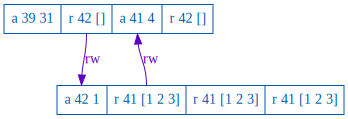
\includegraphics[width=\textwidth]{staleness/32.png}
  \caption{G2-item(сгенерировано Elle)}
\end{figure}
\par

\begin{lstlisting}[caption={Пояснение к G2-item аномалии (сгенерировано Elle)}]
Let:
  T1 = {:type :ok, :f :txn, :value [[:append 42 1] [:r 41 [1 2 3]] [:r 41 [1 2 3]] [:r 41 [1 2 3]]], :time 89283544982, :process 2, :index 7317}
  T2 = {:type :ok, :f :txn, :value [[:append 39 31] [:r 42 []] [:append 41 4] [:r 42 []]], :time 89301402301, :process 4, :index 7319}

Then:
  - T1 < T2, because T1 did not observe T2's append of 4 to 41.
  - However, T2 < T1, because T2 observed the initial (nil) state of 42, which T1 created by appending 1: a contradiction!
\end{lstlisting}

\par
Данная аномалия найдена при тестировании с использованием следующих параметров: уровень согласованности - ограниченное устаревание(англ.  \textit{bounded staleness}),  количество потоков - 15, лимит времени на транзакцию - 120 секунд, ограничение на количество элементов по одному ключу - 128,максимальное количество операций в транзакции - 4.
\par
\textit{\textbf{Пояснение}}
\par
Верхняя транзакция считывает документ 42,который оказывается пустым.Также верхняя транзакция добавляет 4 к документу 41. Нижняя транзакция добавляет 1 к документу 42 и считывает документ 41, обнаруживая, что это значения [1 2 3]. Ребра, помеченные \textit{rw,} обозначают антизависимости чтения и записи. Эти транзакции невозможно изолировать: если бы верхняя транзакция выполнялась первой, изолированно, ее запись в документе 41 была бы видна нижней --- и наоборот. Но поскольку эти транзакции не записывались в одни и те же документы, им разрешено (при \textbf{изоляции моментальных снимков}) выполняться одновременно.

\subsubsection{\textit{Пример 2}}
\begin{figure}[H]
  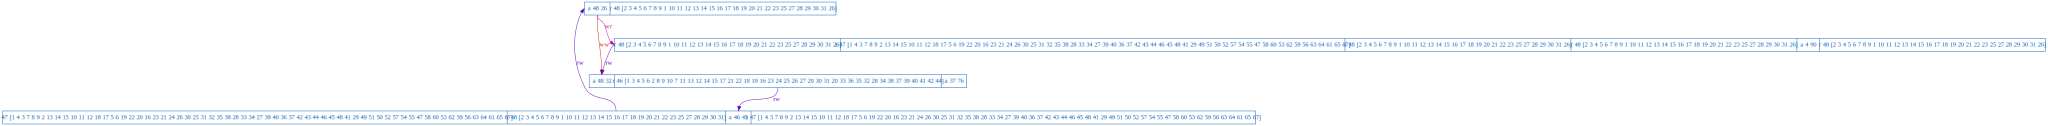
\includegraphics[width=\textwidth]{prefix/7.png}
  \caption{G2-item(сгенерировано Elle)}
\end{figure}
\par
\begin{lstlisting}[caption={Пояснение к G2-item аномалии (сгенерировано Elle)}]
Let:
  T1 = {:type :ok, :f :txn, :value [[:r 48 [2 3 4 5 6 7 8 9 1 10 11 12 13 14 15 16 17 18 19 20 21 22 23 25 27 28 29 30 31 26]] [:r 47 [1 4 3 7 8 9 2 13 14 15 10 11 12 18 17 5 6 19 22 20 16 23 21 24 26 30 25 31 32 35 38 28 33 34 27 39 40 36 37 42 43 44 46 45 48 41 29 49 51 50 52 57 54 55 47 58 60 53 62 59 56 63 64 61 65 67]] [:r 48 [2 3 4 5 6 7 8 9 1 10 11 12 13 14 15 16 17 18 19 20 21 22 23 25 27 28 29 30 31 26]] [:r 48 [2 3 4 5 6 7 8 9 1 10 11 12 13 14 15 16 17 18 19 20 21 22 23 25 27 28 29 30 31 26]] [:append 4 90] [:r 48 [2 3 4 5 6 7 8 9 1 10 11 12 13 14 15 16 17 18 19 20 21 22 23 25 27 28 29 30 31 26]]], :time 84564390536, :process 7, :index 5394}
  T2 = {:type :ok, :f :txn, :value [[:append 48 32] [:r 46 [1 3 4 5 6 2 8 9 10 7 11 13 12 14 15 17 21 22 18 19 16 23 24 25 26 27 29 30 31 20 33 36 35 32 28 34 38 37 39 40 41 42 44]] [:append 37 76]], :time 84573458348, :process 0, :index 5397}
  T3 = {:type :ok, :f :txn, :value [[:r 47 [1 4 3 7 8 9 2 13 14 15 10 11 12 18 17 5 6 19 22 20 16 23 21 24 26 30 25 31 32 35 38 28 33 34 27 39 40 36 37 42 43 44 46 45 48 41 29 49 51 50 52 57 54 55 47 58 60 53 62 59 56 63 64 61 65 67]] [:r 48 [2 3 4 5 6 7 8 9 1 10 11 12 13 14 15 16 17 18 19 20 21 22 23 25 27 28 29 30 31]] [:append 46 45] [:r 47 [1 4 3 7 8 9 2 13 14 15 10 11 12 18 17 5 6 19 22 20 16 23 21 24 26 30 25 31 32 35 38 28 33 34 27 39 40 36 37 42 43 44 46 45 48 41 29 49 51 50 52 57 54 55 47 58 60 53 62 59 56 63 64 61 65 67]]], :time 84560168742, :process 4, :index 5391}
  T4 = {:type :ok, :f :txn, :value [[:append 48 26] [:r 48 [2 3 4 5 6 7 8 9 1 10 11 12 13 14 15 16 17 18 19 20 21 22 23 25 27 28 29 30 31 26]]], :time 84560623148, :process 8, :index 5392}

Then:
  - T1 < T2, because T1 did not observe T2's append of 32 to 48.
  - T2 < T3, because T2 did not observe T3's append of 45 to 46.
  - T3 < T4, because T3 did not observe T4's append of 26 to 48.
  - However, T4 < T1, because T1 observed T4's append of 26 to key 48: a contradiction!
\end{lstlisting}

\par
Данная аномалия найдена при тестировании с использованием следующих параметров: уровень согласованности - постоянный префикс(англ.  \textit{consistent prefix}),  количество потоков - 15, лимит времени на транзакцию - 120 секунд, ограничение на количество элементов по одному ключу - 128, максимальное количество операций в транзакции - 7.

\textit{\textbf{Пояснение}}
\par
Это более сложный цикл, состоящий из 4 транзакций.  Каждая из этих транзакций зависит от другой. Ребра с надписью \textit{ww} показывают зависимость записи от записи, при которой одна транзакция перезаписывает запись другой. Те ребра, на которых написано \textit{wr}, показывают зависимость запись-чтение: одна транзакция считывает запись другой.

\subsection{G2-item: \textit{что это значит?}}
Итак, давайте разберемся, что означает найденная аномалия. Заметим, что в документации Azure Cosmos DB сказано, что транзакции полностью атомарны, изолированы,согласованы и прочны(<<\textit{full ACID}>>).  Однако это не совсем так, потому что транзакции, поддерживающие \textbf{изоляцию моментальных снимков} не являются полностью изолированными. 
\par
То есть, полученные нами истории, по-видимому, не нарушают \textbf{изоляцию моментальных снимков}, но, тем не менее, демонстрируют циклические зависимости транзакций.
\par
Можно ли говорить, что эти истории удовлетворяют требованиям <<\textit{full ACID}>>? Возможно, но если это так, тогда следует также признать, что <<\textbf{I}>> в \textit{ACID} означает только частичную изоляцию, или <<\textit{full}>> означает несколько меньше, чем полная.
\par
Данная аномалия не редкость. Примерно в 15\% транзакций наблюдались аномалии во время нормальной работы, без сбоев.

\subsection{Грязное обновление (англ. \textit{Dirty Update})}
Довольно редкая аномалия. Она встретилась в менее чем 1 \% транзакций.
\par
Данная аномалия найдена при тестировании с использованием следующих параметров: уровень согласованности - ограниченное устаревание(англ.  \textit{bounded staleness})  количество потоков - 5, лимит времени на транзакцию - 60 секунд, ограничение на количество элементов по одному ключу - 256, максимальное количество операций в транзакции - 4.
\par
\textit{Описание}: по ключу 4 транзакция T1 пыталась добавить значение 4, во время выполнения транзакции произошла ошибка и статус операции был определен как fail. Транзакция T2 далее записала по ключу 4 значение 5.  Далее другие транзакции увидели по ключу 4 значения [4 5].

\subsection{G1a: прерванное чтение(англ. \textit{Aborted read})}
Довольно редкая аномалия. Она встретилась в менее чем 1 \% транзакций.
\begin{lstlisting}[caption={Пример G1a аномалии}]
{:op {:type :ok,
	:f :txn,
	:value [[:append 9 145]
		   [:r 6 [1 2 3 4 5 6 7 8 9 10]]],
	:time 27666818490,
	:process 2,
	:index 501},
 :mop [:r 6 [1 2 3 4 5 6 7 8 9 10]],
 :writer {:type :fail,
	     :f :txn,
	     :value [[:r 8 nil]
		        [:append 4 4]
		        [:append 6 8]],
	     :time 24489725317,
	     :process 3,
	     :error :cosmos-exception,
              :index 463},
 :element 8}
\end{lstlisting}
\par
Данная аномалия найдена при тестировании с использованием следующих параметров: уровень согласованности - ограниченное устаревание(англ.  \textit{bounded staleness})  количество потоков - 5, лимит времени на транзакцию - 60 секунд, ограничение на количество элементов по одному ключу - 256, максимальное количество операций в транзакции - 4.

\subsection{G1a и Dirty Update: \textit{что это значит?}}
В документации Azure Cosmos DB сказано, что если в процессе исполнения JavaScript программы происходит исключение, тогда вся транзакция прерывается и выполняется откат.Ожидается, что эти отброшенные изменение не будут видимы.
\par
Однако в данных случаях мы получили сообщение об ошибке в транзакции, но она не была прервана и не был выполнен откат измененных ею данных.
\par
Также следует отметить, что все замеченные \textit{G1a} и \textit{Dirty Update} аномалии произошли на уровне согласованности ограниченное устаревание(англ.  \textit{bounded staleness}) и попали в <<окно устаревания>>.  

\chapter{Выводы}
В данной работе был обозначен ряд проблем, которые возникают в распределенных системах. Зачастую они носят случайный характер. Также их сложно выявить на этапе разработки распределенной системы.  Это обуславливает необходимость введения формальных определений различных моделей согласованности.
\par Также сложность обнаружения различный нарушений изоляции и согласованности обуславливает появление Jepsen как интструмента для проверки гарантий выполнения важнейших свойств распределенных систем. С этим инструментом мы познакомились в данной работе.
\par Кроме того, в этой работе мы попробовали самостоятельно проанализировать реальную базу данных --- Cosmos DB.  Cosmos DB утверждает, что поддерживает  <<полностью ACID транзакции>> через изоляцию моментальных снимков. Однако использование этих транзакций осложняется запутанной документацией и API.  А также изоляция моментальных снимков плохо совместима с маркетинговой фразой <<\textit{full ACID}>>.  Мы регулярно наблюдали истории, которые казались совместимыми с изоляцией моментальных снимков, но также включали сотни аномалий G2-item (циклы анти зависимости), в которых транзакции не наблюдали эффектов друг друга. Это нормально и разрешено при изоляции моментальных снимков, но являются ли эти транзакции полностью изолированными  в смысле \textit{ACID}? Это спорно.
\par Итак, в этой работе мы провели лишь краткое исследование. В дальнейшем в рамках развития данной работы возможно реализовать другие тесты, например, \textit{register} тест, а также исследовать поведение базы данных при различных сбоях.


\bibliographystyle{unsrt}
\bibliography{references}


\end{document}
